\chapter{Timing}
\label{chap:timing}
\section{What is timing}

    Mechanisms for measuring time are found in a variety of organisms, from humans to plants \cite{cashmore2003cryptochromes}. Initially bound by external rhythms (like circadian cycles), time estimation mechanisms were among the first competencies evolved in biological systems \cite{paranjpe2005evolution}, and are constitutive of many other cognitive modalities such as decision making and episodic memory \cite{maniadakis2014time}. Most behaviors are inseparable from their temporal or rhythmic component \cite{buhusi2005makes}. From deciding to accelerate or break in yellow light, through the simple motor organization of walking or running, to the complex dynamics of speech and musical performance, computational processes conducted by the brain must be temporally structured to ensure correct execution \cite{bueti2014temporal}. 
    
    \begin{figure}
        \centering
        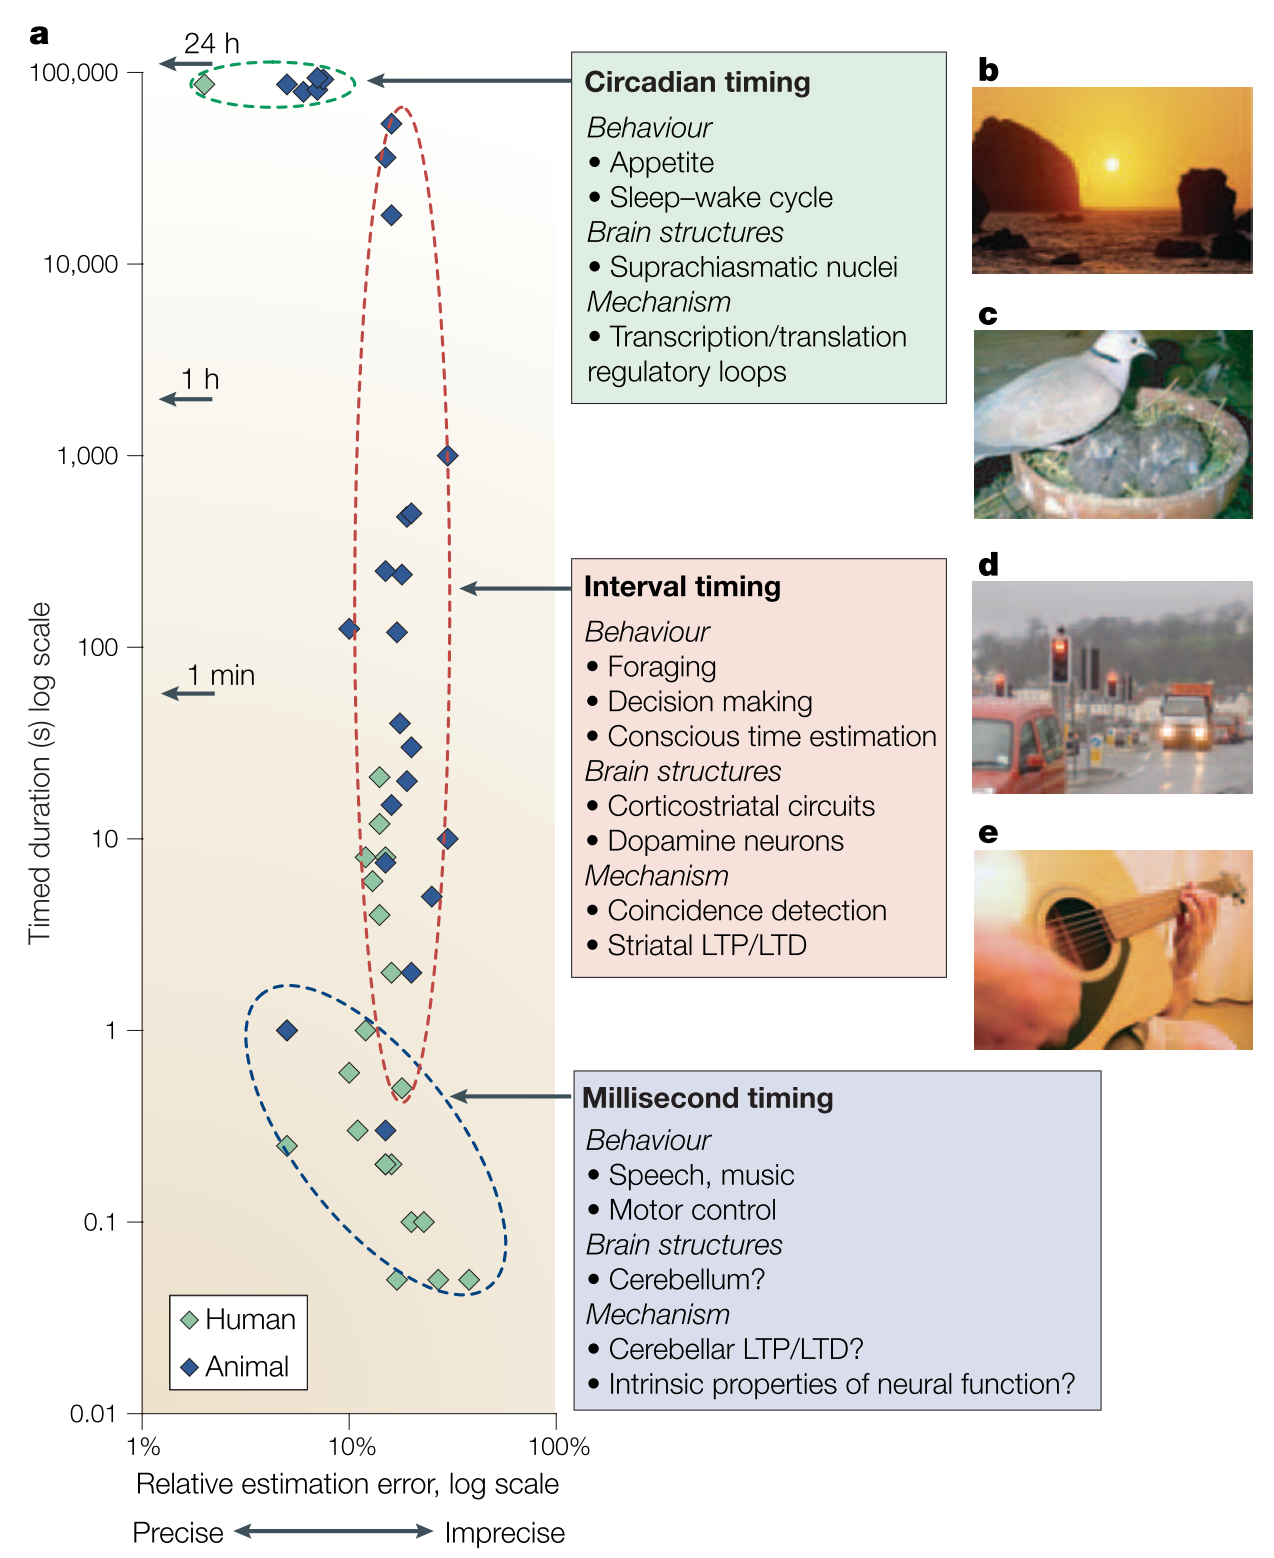
\includegraphics[width=.95\textwidth]{figures/sketches/timescales.png}
        \caption[Timing across different timescales.]{Timing across different timescales. a) Studies compiled from various sources, divided into three groups. Precision of estimations depends on the time scale. While (b) Circadian rhythms are related to natural cycles of sunlight, behavior like (c) coordinating egg incubation is guided by interval-timing in male doves, as well as d) decision making in humans, such as stopping or accelerating in a yellow light. e) Millisecond timing is central to the playing of music. Taken from Buhusi and Meck \cite{buhusi2005makes}}
        \label{fig:timescales}
    \end{figure}
    
    While organisms and their brains have to account for event durations in many timescales, from milliseconds to days, there is no single neural correlate proved to account for them all \cite{buhusi2005makes, buhusi2016clocks, hardy2016neurocomputational, lewis2003distinct, mauk2004neural}. On the one hand, circadian rhythms depend on the suprachiasmatic nucleus (SCN), relying on slow protein cycles managed by transcriptional feedback loops \cite{buhusi2005makes}, and are important to regulate social and foraging behavior. In turn, the temporal structure of milliseconds relies on local circuits and their communication with the cerebellum \cite{ohmae2017cerebellar}, and is essential to fine motor control, such as playing an instrument or making a tool. In between, the time scale of seconds is central to planning, decision making, and reasoning \cite{buhusi2005makes}, and is dependent on the Striatum \cite{mello2015scalable}, but independent of the SCN \cite{lewis2003interval} and cerebellum \cite{harrington2004does}. The present work focuses on the scale of seconds, namely \textit{interval timing}.
    
\section{The anatomy of timing}
\label{sub:anatomy}
     %Accordingly, the scale of seconds to minutes is categorized as \textit{Interval Timing}, and its properties can be assessed through a variety of tasks \cite{lloyd2012neural,astrand2014comparison,brea2016prospective,mello2015scalable,gouvea2015striatal,kopec2018controlling,gershman2014dopamine,tiganj2016sequential,narayanan2009delay,cho2010differential}.
    The scale of seconds is less well-understood than its counterparts, but there is plenty of experimental evidence about regions and mechanisms likely involved in interval estimation over this scale. Evidence comes from a variety of experimental modalities, from psychophysics \cite{ohmae2017cerebellar} and pharmacology \cite{pine2010dopamine, meck2012gene, drew2003effects, cheng2016clock, ludvig2008stimulus} to lesion studies \cite{meck2006frontal} and electrophysiology \cite{bakhurin2017differential}. Psychophysical studies consistently report that time estimation obeys Weber's law \cite{gibbon1977scalar}, that is, the error in responses is proportional to the mean estimated duration, and thus time-scale invariant. From pharmacology, we know that dopamine agonists shorten time estimates \cite{cheng2016clock, pine2010dopamine} while antagonists elongate them \cite{drew2003effects}; Lesion studies show that some regions (e.g. Striatum, PFC, Hippocampus) are necessary for timing behavior \cite{cho2010differential};
    Lastly, electrophysiology provides suggestions of neural correlates of timing, such as ramping neurons in the PFC \cite{kim2013neural}, time cells in the mPFC \cite{tiganj2016sequential} and Hippocampus \cite{eichenbaum2014time}, and the Contingent Negative Variation in EEG \cite{pfeuty2005relationship}.
     
    Even though the neural structures necessary for successful performance differ between the various Interval Timing tasks \cite{paton2018neural}, it cannot be ruled out the possibility of a single underlying neural mechanism rendering the time representation \cite{gibbon1977scalar}, or still further a single region for Interval Timing common to all mechanisms \cite{mello2015scalable}. Some common properties shared across different tasks support this idea of a single mechanism underpinning all timing in the order of seconds \cite{buhusi2005makes, gibbon1977scalar}. For example, the scalar property is present as a crucial feature of many models \cite{gibbon1977scalar, oprisan2014all}. The reliance on the dopamine system to optimal performance is also featured among various timing tasks and often taken into consideration for the development of timing models \cite{kim2017optogenetic, meck2012gene}.
    
    Independently of how dedicated or intrinsic are time representations, an important role is traced to cortico-striatal circuits \cite{lusk2016utilizing, buhusi2005makes, meck2008cortico}, in special to the mPFC \cite{buhusi2018inactivation} and the Striatum \cite{mello2015scalable}.
    
    \subsection{Medial Pre-Frontal Cortex}

        The medial prefrontal cortex has been implicated in Timing based in multiple tasks, such as Reaction Time \cite{narayanan2009delay}, Differential Reinforcement of Low rate \cite{cho2010differential} Temporal Bisection \cite{kim2009inactivation,tiganj2016sequential,kim2013neural}, and Peak Procedure \cite{buhusi2018inactivation}. Its implication in timing has also been revealed through distinct methods, such as lesions \cite{cho2010differential}, inactivation by muscimol \cite{buhusi2018inactivation, kim2009inactivation}, and optogenetic stimulation \cite{kim2017optogenetic}. 

    \subsection{Striatum}
        The Striatum is a part of the basal ganglia, a series of subcortical nuclei that connect both to Cortex and Brainstem \cite{helie2015learning}. This structure has been traditionally associated with procedural learning, and with the initiation and termination of movements \cite{helie2015learning}. Malfunction of the basal ganglia may lead to neurological diseases, such as Parkinson's, in which patients' erratic movements and trembling indicate their deregulation due to a lack of dopamine \cite{buhusi2005makes}.    
        
        Animals require an intact Striatum for the appropriate performance of many Interval Timing tasks \cite{mello2015scalable,gouvea2015striatal,cho2010differential}. Accordingly, many timing models place it as a central structure \cite{mello2015scalable, buhusi2005makes}.
        
    \subsection{The taxonomy of timing}
    \label{sub:taxonomy}
    
        % The split between explicit and implicit memory was a breakthrough, providing a framework that enabled new kinds of questions \cite{paton2018neural}. % Change, explain
        % The scale of seconds has a name, but not clear boundaries. 

        Studies often use the scale of time intervals as the single distinction between experiments \cite{van20168, buhusi2005makes, hardy2016neurocomputational}, but there is no consensus on exact boundaries between timing scales. In figure \ref{fig:timescales}, it is possible to see overlap between the millisecond timing and interval timing scales, specifically close to the order of one second. What constitutes a single timing mechanism may range from seconds to minutes in some studies \cite{mello2015scalable}, and from tens to hundreds of milliseconds in others \cite{mauk2004neural}. One of the difficulties in delineating specific boundaries is the fact that mechanisms may not depend solely on the time interval, but also depend on other task characteristics \cite{lewis2003distinct}.
        
        The field of timing currently lacks a thorough taxonomy, to group forms of timing that depend on similar circuits and mechanisms, and distinguishing those that do not \cite{paton2018neural}. Paton and Buonomano \cite{paton2018neural} proposed one such grouping, to be used as a starting point in the creation of this timing taxonomy. They considered the computational requirements of many tasks and arrived at a three-dimensional account for them.
        \begin{enumerate}
            \item \textit{Subsecond vc Suprasecond timing}. The most established dimension in the study of timing, intervals in the low hundreds of miliseconds seem to require distinct regions compared to multiple seconds. 
            \item \textit{Motor vs Sensory timing}. Distinguishes tasks in which motor responses have to be timed from those where responses are only decisional such as interval comparison.
            \item \textit{Interval vs Pattern timing}. Timing tasks that depend on sequential intervals, such as music and speech, are distinct from single intervals.
        \end{enumerate}
        
        The importance of delineating a taxonomy should not be understated. When the study of memory made the distinction between explicit and implicit memories, it enabled the raising of a whole new set of questions \cite{paton2018neural}. Currently, models of time refer to single mechanisms, and a better taxonomy could facilitate their application.

\section{Timing models}
\label{sec:models}
    The Scalar Expectancy Theory (SET) proposes a model, schematized in figure \ref{fig:set_schema} where a counter achieves timing, accumulating pulses from a pacemaker and comparing them with reference memories \cite{gibbon1977scalar}. Despite the simplicity, the model fits psychophysical data from the most common timing tasks \cite{machado2009learning} correctly predicting time-scale invariance and explaining the effect of dopamine as an accelerator of the pacemaker.
    
    \begin{figure}
        \centering
        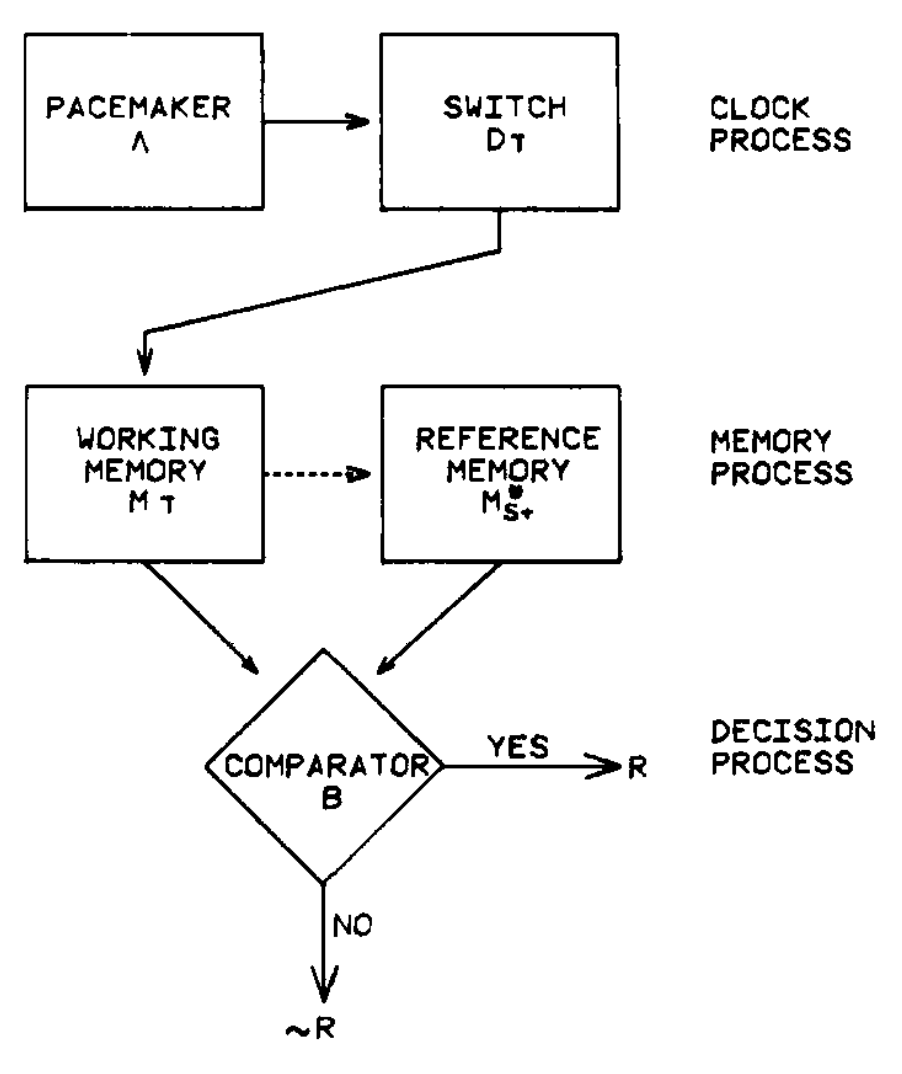
\includegraphics[width=5cm]{figures/SET_model_schema.png}
        \caption[The SET model of timing.]{Sketch of the SET model of timing. Taken from \cite{gibbon1977scalar}.}
        \label{fig:set_schema}
    \end{figure}
    
    The SET model is by far the most popular timing model \cite{buhusi2005makes}, having retained attention from the community for more than 30 years. Even though it has limitations and fails to predict some results \cite{machado2009learning}, its simplicity seems to compensate for it. There are too many timing models to consider an exhaustive listing, and we introduce those that best foster our examination across levels of analysis. 
    
    In terms of algorithm, it has been shown that Drift Diffusion Models (DDMs) are a more general framework that encompasses the SET, LET, and other common models \cite{balci2016decision}. DDMs are evidence-accumulation models, that compare the evidence among two alternatives in a noisy setting, and are optimal in the sense they can reach some predetermined accuracy in the least amount of time. They have the interesting uptick of being commonly used to study decision making, and thus frame timing in terms of decision. 
    
    \begin{figure}
        \centering
        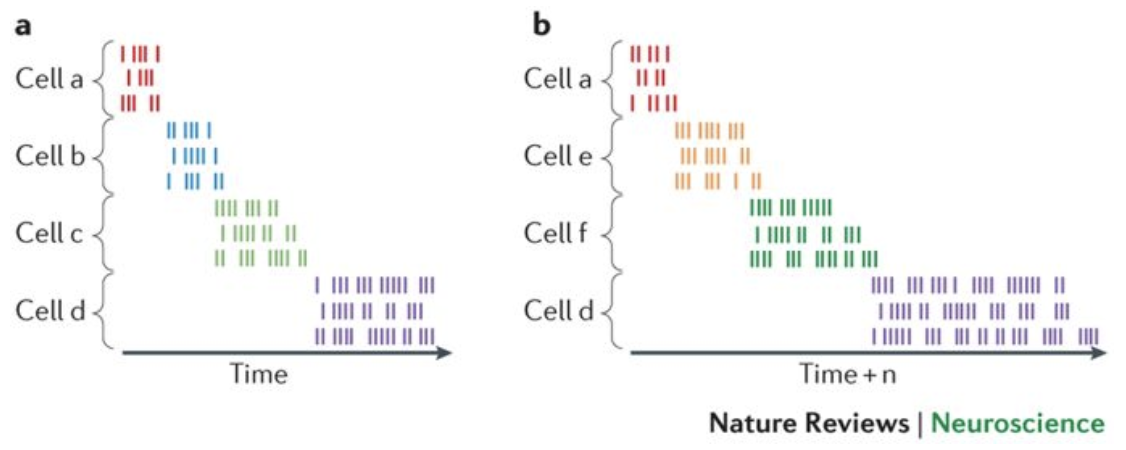
\includegraphics[width=0.95\textwidth]{figugres/sketches/time_cells.png}
        \caption[Time cells]{Time cell. a | Each cell has a temporal receptive field, firing preferentially at some point in time. b | When the interval is increased, time cells change their preferential time. \cite{eichenbaum2014time}.}
        \label{fig:timecells}
    \end{figure}

    \begin{figure}[ht]
        \centering
        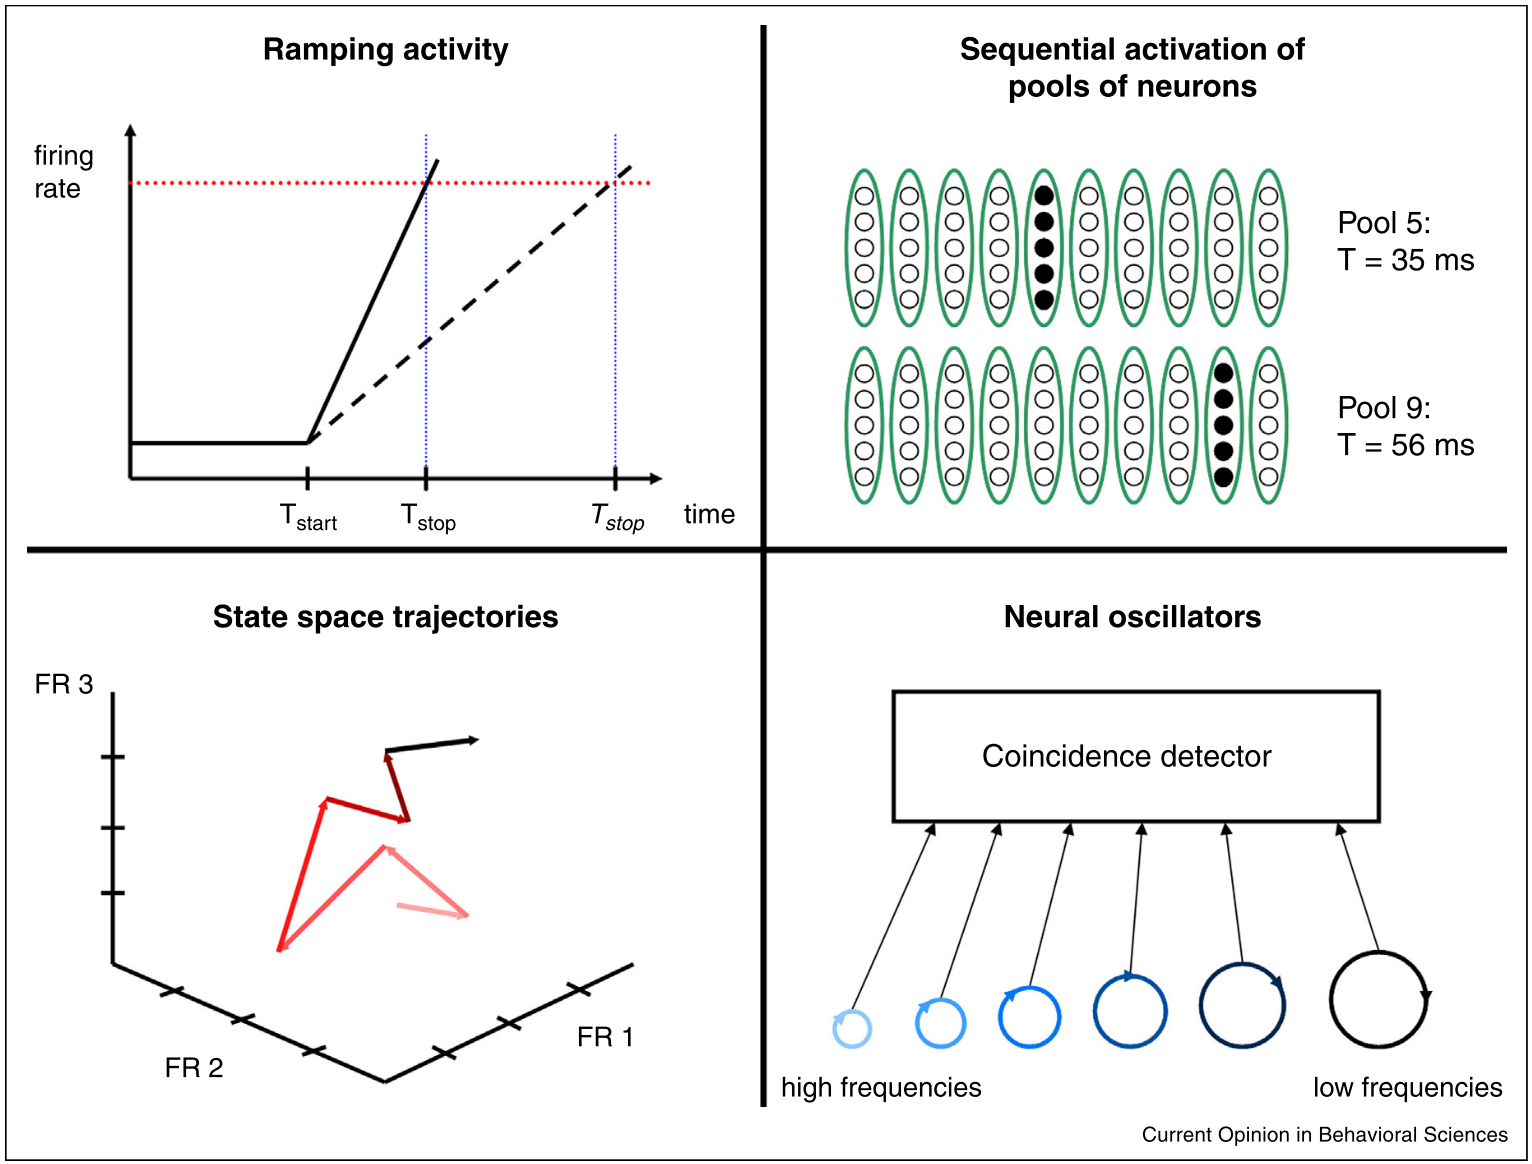
\includegraphics[width=\textwidth]{figures/sketches/kinds_of_timing_models.png}
        \caption[Mechanisms of time perception]{Mechanisms of time perception, according to Hass and Durstewitz \cite{hass2014neurocomputational}. Four distinct implementations for time representation are depicted. Explaining clockwise: Ramping activity models pose that time is encoded in the instantaneous firing rate of ramping neurons. Synfire chains pose that pools of neurons, connected in a feedforward manner, encode time in the ordinal position of the active neuron pool. Neural oscillator models propose that coincidence detectors in the brain can be used to reliably encode time intervals much larger than the interval of neural oscillators being compared. Finally, State space trajectories make less assumptions, posing that time is encoded trajectories of population activity (and other state variables such as short term plasticity).}
        \label{fig:my_label}
    \end{figure}

    At the level of implementation, the most discussed model is simply the ramping neuron \cite{hass2014neurocomputational}, where single neurons increase their activity up to a threshold that triggers the response. Single neuron models also feature time cells \cite{tiganj2016sequential}, whose activity marks a point in time. Alternatively, there are a variety of state-dependent network models (SDNs), where time is represented in the collective activity of many neurons \cite{hardy2016neurocomputational}. A specific case, "synfire chains" model sequentially activated cell assemblies \cite{paton2018neural}.
    
    In the halfway between algorithm and implementation, neural oscillation models are based on experimental data regarding neuronal activity that could be managed in specific ways. The main example, the Striatal Beat Frequency model \cite{mello2015scalable}, proposes that the Striatum has the hardware to implement a coincidence detection algorithm, able to reach regular patterns in much longer timescales than the regular patterns we call oscillations. Of the examples we presented, state-dependent networks are the most general: all of the other models can be interpreted as particular cases of SDNs \cite{hass2014neurocomputational}. However, instances of SDN proposed in the literature generally emphasize that trajectories in the phase space are intricate, in opposition to the elementary ones that could be represented by the simpler models \cite{buonomano2009state}.

    There are many attempts to bridge the gap between Algorithm and Implementation, one of which is proposed by Simen et al. \cite{simen2011model}. They build up from individual neurons to a DDM, by successive approximations, at last showing one manner of implementing DDMs in biological networks of neurons. While ample evidence has been provided in the context of behavioral performance in timing, the mechanisms through which the correct behavior develops during learning are much less frequently studied \cite{van20168}. 

\section{Learning}
\label{sec:learning}
    \subsection{Instrumental learning}
        The literature identifies two distinct forms of behavior linked to learning. One is goal-directed, in which the animal knows the consequence of its action (belief), and wants that consequence (desire). The other is habitual, in which the animal is insensitive either to belief or desire, acting in a predetermined manner. Take the example of pressing a lever for food pellets: if the animal is not hungry (no desire) or the lever stops yielding access to food pellets (no belief), it will stop pressing if the behavior was goal-directed, but continue pressing if it was habitual \cite{dickinson2015instrumental}. In sum, while goal-directed behavior is flexible to changes in reward schedules, habitual behavior is resistant to changes in environmental contingencies \cite{dickinson2015instrumental}.
        
        Beyond the belief-desire account, we can frame the dual systems in terms of associations: While Response-Outcome (RO) associations give rise to Goal-directed behavior, Stimulus-Response (SR) associations give rise to habitual behavior \cite{dickinson2015instrumental}. Connecting to the belief-desire account, we can note that Response-Outcome associations connect the consequences (outcomes) to the actions (responses), so the belief that some outcome is consequent of the response is encoded in the associations. In turn, Stimulus-Response associations have no reference to the outcome, and are thus unaffected by changes in desire to the outcome.
        
        One third frame is in terms of reinforcement learning: model-based learning corresponds to goal-directed behavior while model-free learning is habitual \cite{decker2016creatures}. In Reinforcement Learning, "model" refers to the a transition function $P: S\times A \rightarrow S$ related to taking actions in the environment. Taking the action $a$ at a given state $s$ changes the state to $P(s, a)$, for example pressing the left lever when the light is green makes the reward available. In model-based learning animals learn the model of the environment, that gives the outcomes for each action, and use this models to decide how to act and maximize their reward (if they so desire). In turn, in model-free learning animals learn the value of actions for each state, without reference to the consequences of the actions.
        
        %Based on a model $P$, it is possible to calculate the optimal policy, 
        Each system has its own neurobiological substrate: while the goal-directed depends on the dmPFC and the dSTR, the automatic depends on the vmPFC and the vSTR \cite{dickinson2015instrumental}. 

    \subsection{Training may change neural substrates}
        Studies on the corticostriatal role in decision making have already proposed the coexistence of two heterogeneous learning processes \cite{balleine1998goal, balleine2007role, smith2013dual}: one of them consists of an automatic/habitual Stimulus-Response learning, strengthened by reinforcers, while the other reflects a goal-directed/flexible Response-Outcome learning \cite{dickinson2015instrumental}. The neurobiological substrates of these two processes have been dissociated, wherein the goal-directed is dependent on dmPFC and dorsal Striatum, and the automatic is dependent on vmPFC and ventral Striatum \cite{dickinson2015instrumental}. Studies on the vmPFC's importance to learning, in the field of fear extinction, point out to its role in retaining learning \cite{phelps2004extinction}, while it seems necessary to performance in gambling tasks \cite{rogalsky2012risky}. Distinctly, dmPFC's role has been verified to bolster learning but not performance \cite{balleine2007still}.

        As exemplified in the previous subsection, either the goal-directed or habitual systems can control the same behavior. What is especially relevant to the present work is the role of training in this control -- it depends on the extent of training of the subject. Generally, over-training makes a behavior habitual, or more specifically: makes the habitual system the main controller of behavior \cite{dolan2013goals}. While the amount of training may change the main controller from goal-directness to habitual, this effect is task-dependent. Complex tasks are hard to automate, while unpredictable reward schedules make the task harder to control in a goal-directed manner. Both systems work conjointly to guide behavior, with their relative contribution dependent on the reinforcement schedule in addition to the complexity of the task \cite{dickinson2015instrumental}.
        
    \subsection{Learning to time}
        While this general mechanisms have been proposed to Instrumental Learning in general, they have been largely neglected by the timing community, which focuses mainly on the representation. Moreover, much of the work in Timing has focused on well-trained subjects \cite{bakhurin2017differential}, what limits the ability to select models. 
        
        The SET model \cite{gibbon1977scalar} has a simple account for enhancement of interval representations with training. Each time the decision process correctly reaches a reward, the current time representation is aggregated in long term memory, that stores the mean of rewarded times. This stored reference is used for compatrison with new intervals, and the similarity between the perceived and reference intervals is used to guide subsequent responses. 
        
        The LeT model \cite{machado2009learning}, connectionist in nature, places the learning process in the connections between states and actions. Rewards received by the animal strengthen those connections active at the moment of reward, and weaken those inactive. Hence, after attaining some rewards, states corresponding to the criterion time have their connections strengthened, making the animal likely to act in these states. In opposition, states corresponding to intervals shorter or longer than the criterion have weaker connections, making the animal less prone to respond.
        
        The dual-systems perspective, although established in the instrumental learning community, does not figure yet in the timing literature, and it may be important to our present work, since we study the neural activity during training. 
    